\documentclass[12pt,a4paper]{article}

% --- Paquetes ---
\usepackage[utf8]{inputenc}
\usepackage[T1]{fontenc}
\usepackage{lmodern}
\usepackage{geometry}
\usepackage{setspace}
\usepackage{parskip}
\usepackage{hyperref}
\usepackage{graphicx}
\usepackage{xcolor}
\usepackage{float}

% --- Configuración de página ---
\geometry{margin=2.5cm}
\onehalfspacing

% Si se quiere eliminar, se tiene que quitar tambien las configuraciones del style.cls
% \fancyhead[L]{ % Encabezado a la izquierda
%   \begin{picture}(0,0) \put(-40,16){
\includegraphics[width=15mm]{img/logo-uc-3.pdf}} \end{picture}
%   \put(8,40){\textcolor{gray}{\scriptsize{\begin{tabular}{l}
%     PONTIFICIA UNIVERSIDAD CATÓLICA DE CHILE\\
%     FACULTAD DE MATEMÁTICAS\\
%     DEPARTAMENTO DE ESTADÍSTICA
%   \end{tabular}}}}
% }

% \pagestyle{fancy}
% \setlength{\headheight}{54pt}
% \renewcommand{\headrulewidth}{0pt}

\csname title\endcsname{Tarea 1 - EYP3707}
\author{Juan Pablo Cuevas}
\date{Mayo, 2026}

\begin{document}
\maketitle

\section{Estadística descriptiva}

Para realizar la estadística descriptiva, se seleccionó un subconjunto de variables relevantes respecto a la correlación con la variable respuesta \texttt{log\_comments}. En la Tabla \ref{fig:correlaciones} se presentan las primeras 20 variables con mayor correlación (mayor a 0.4).

\begin{figure}[H]
    \centering
    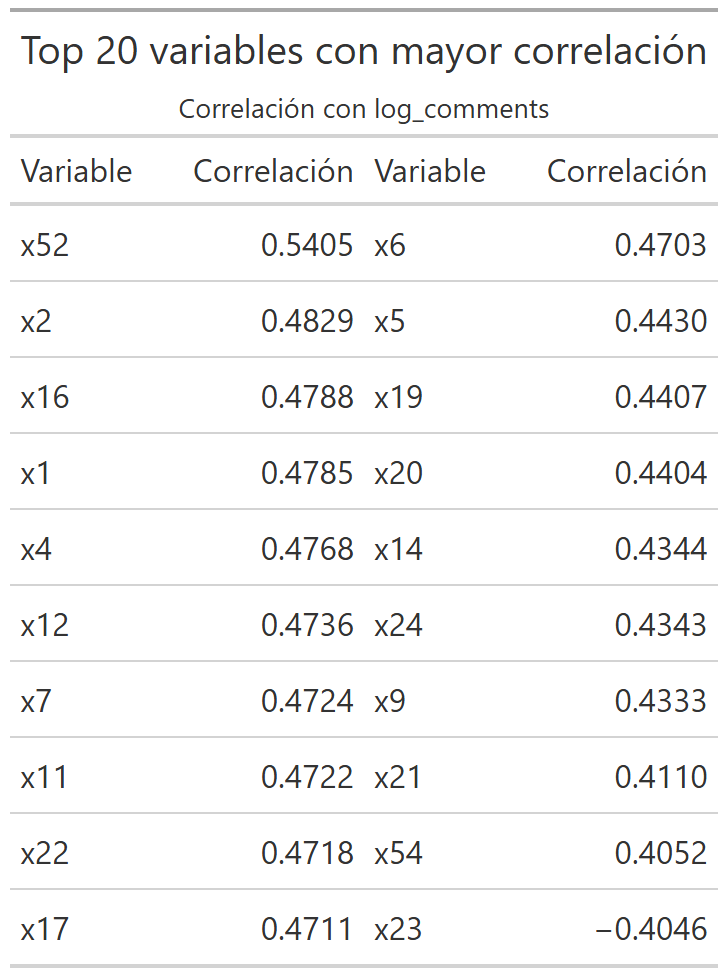
\includegraphics[width=0.5\textwidth]{tabla_correlaciones.png}
    \caption{Matriz de correlación entre variables seleccionadas.}
    \label{fig:correlaciones}
\end{figure}

Descartamos la posibilidad de multicolinealidad de las variables con la variable respuesta, ya que no se observa una correlación alta (máximo de 0.54, que corresponde a la variable x52). Notamos que la variable x23 es la única que presenta una correlación negativa con la variable respuesta, por lo tanto se puede asumir que su aumento afectará a la cantidad de comentarios recibidos en las próximas 24 horas.

Realizamos Tabla \ref{fig:estadistica_descriptiva} con medias, desviaciones estándar, mínimos y máximos para cada una de las variables seleccionadas.

\begin{figure}[H]
    \centering
    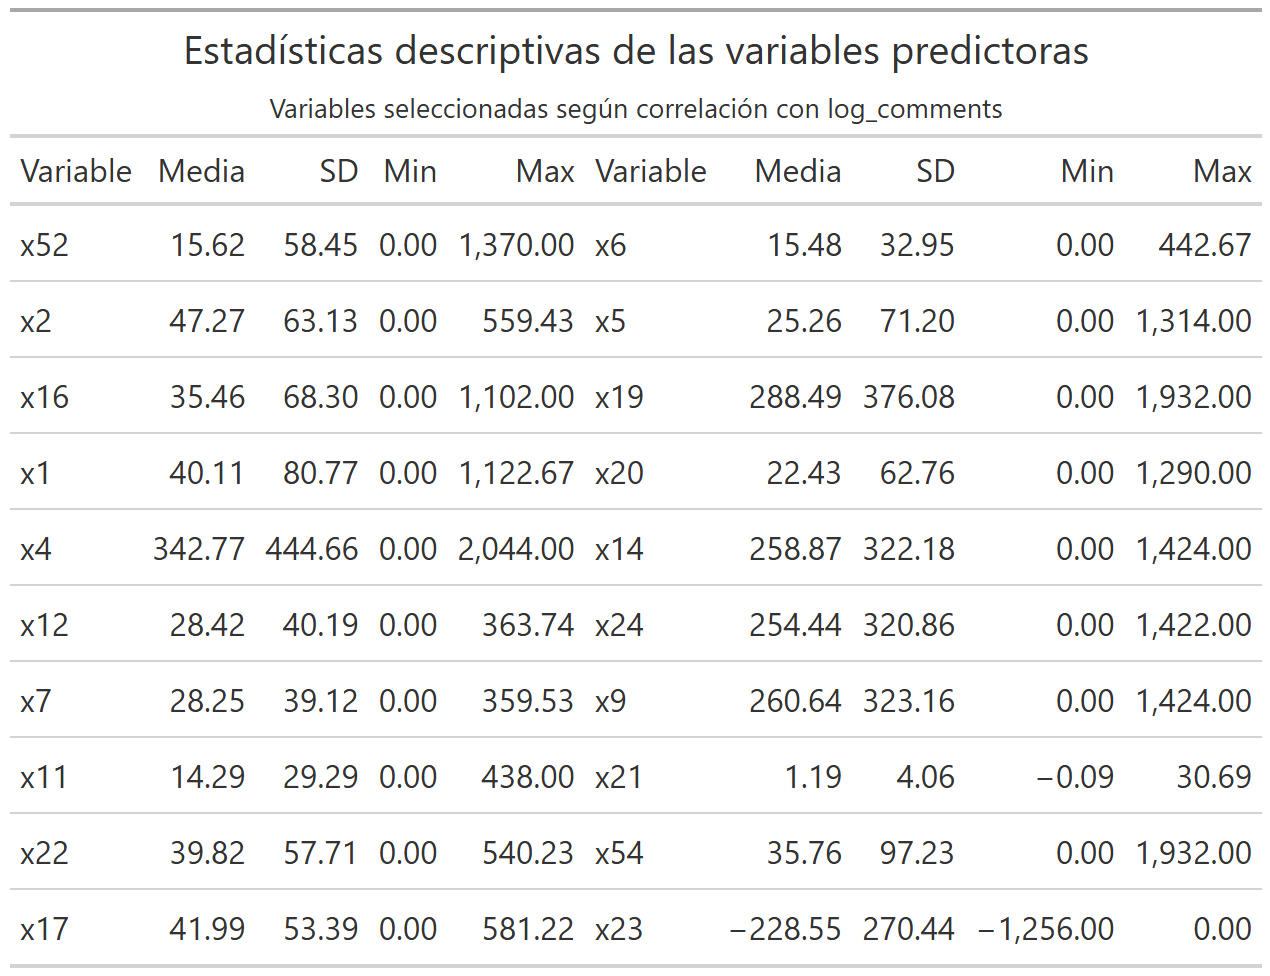
\includegraphics[width=0.85\textwidth]{tabla_descriptiva.png}
    \caption{Estadística descriptiva de las variables seleccionadas.}
    \label{fig:estadistica_descriptiva}
\end{figure}

De la Tabla \ref{fig:estadistica_descriptiva} se observa que las variables presentan distintos comportamientos, con algunas variables que presentan una media cercana a cero y otras con medias más altas. Además, se pueden observan diferencias significativas entre las desviaciones estándar de las variables, lo que indica que algunas variables tienen una mayor dispersión que otras. Esto es debido a que representan diferentes aspectos de los datos.

Realizamos la tabla para la variable respuesta \texttt{log\_comments}.

\begin{figure}[H]
    \centering
    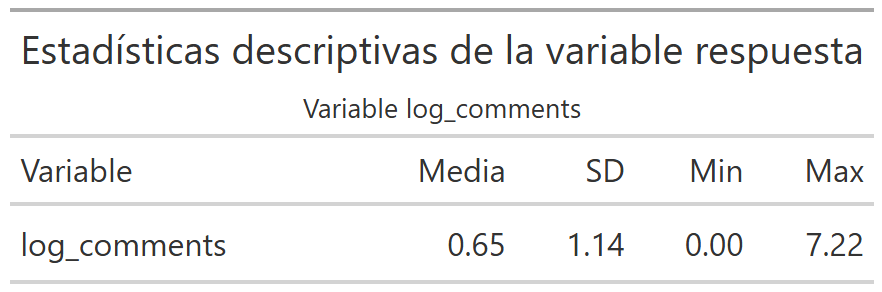
\includegraphics[width=0.6\textwidth]{tabla_descriptiva_logcom.png}
    \caption{Estadística descriptiva de la variable respuesta \texttt{log\_comments}.}
    \label{fig:log_comments_descriptiva}
\end{figure}

De lo visto en la Tabla \ref{fig:log_comments_descriptiva}, la media y la desviación estándar de la variable respuesta \texttt{log\_comments} indican que la mayoría de los comentarios recibidos en las próximas 24 horas se encuentran en un rango relativamente bajo, aunque hay algunos casos que puede existir una cantidad significativa de comentarios.

Incluimos gráfico de correlación entre las variables seleccionadas y la variable respuesta. El gradiente de la derecha indica la intensidad de la correlación, donde el rojo representa una correlación positiva, el azul una correlación negativa y el blanco una correlación cercana a cero.

\begin{figure}[H]
    \centering
    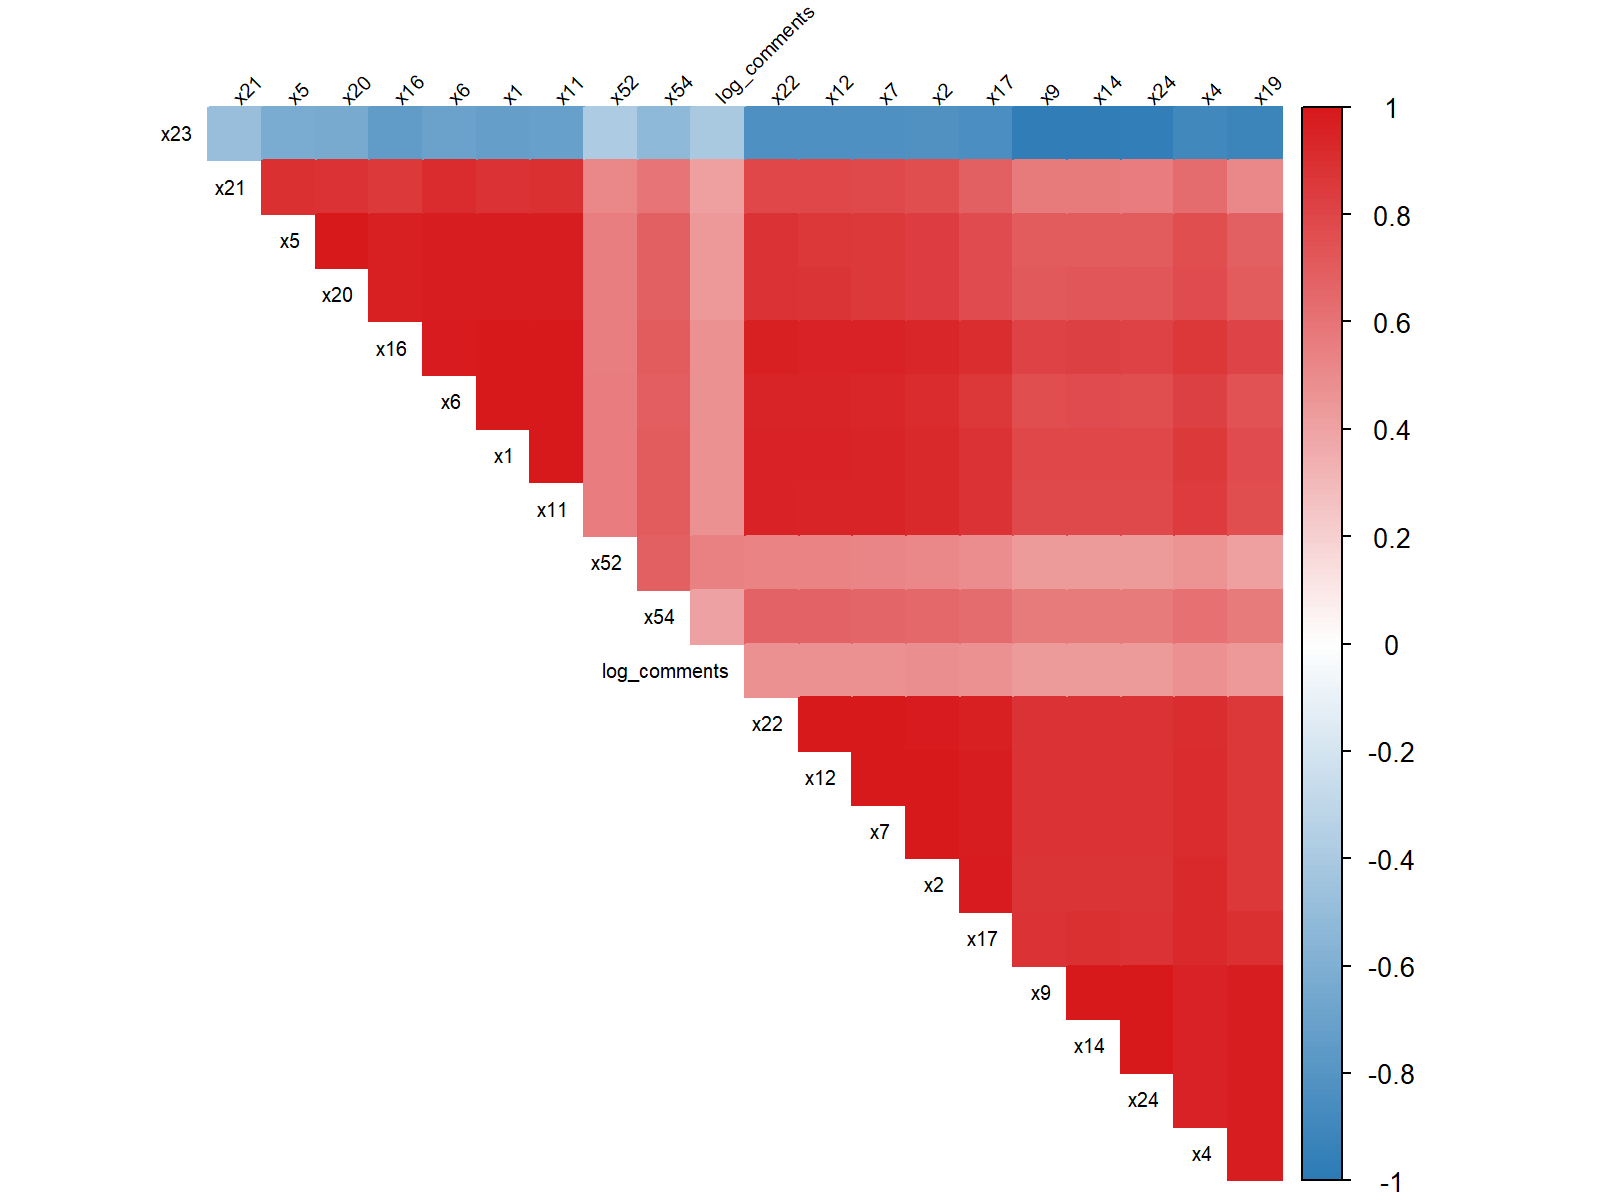
\includegraphics[width=0.95\textwidth]{corrplot_variables.png}
    \caption{Gráfico de correlación entre las variables seleccionadas y la variable respuesta \texttt{log\_comments}.}
    \label{fig:correlacion_log_comments}
\end{figure}

De la Figura \ref{fig:correlacion_log_comments} notamos una alta correlación entre varias variables explicativas, lo que sugiere la presencia de multicolinealidad. Por otro lado, la variable respuesta \texttt{log\_comments}   presenta correlaciones moderadas o bajas con la mayoría de las variables, lo que indica que ninguna variable por sí sola explica fuertemente su comportamiento.

A diferencia de lo anterior, la variable x23 presenta una correlación baja o cercana a cero con la mayoría de las variables, e incluso en algunos casos una correlación negativa débil, demostrando que su comportamiento es relativamente independiente del resto.

Presentamos histogramas para cada una de las variables seleccionadas, con el fin de visualizar su distribución.

\begin{figure}[H]
    \centering
    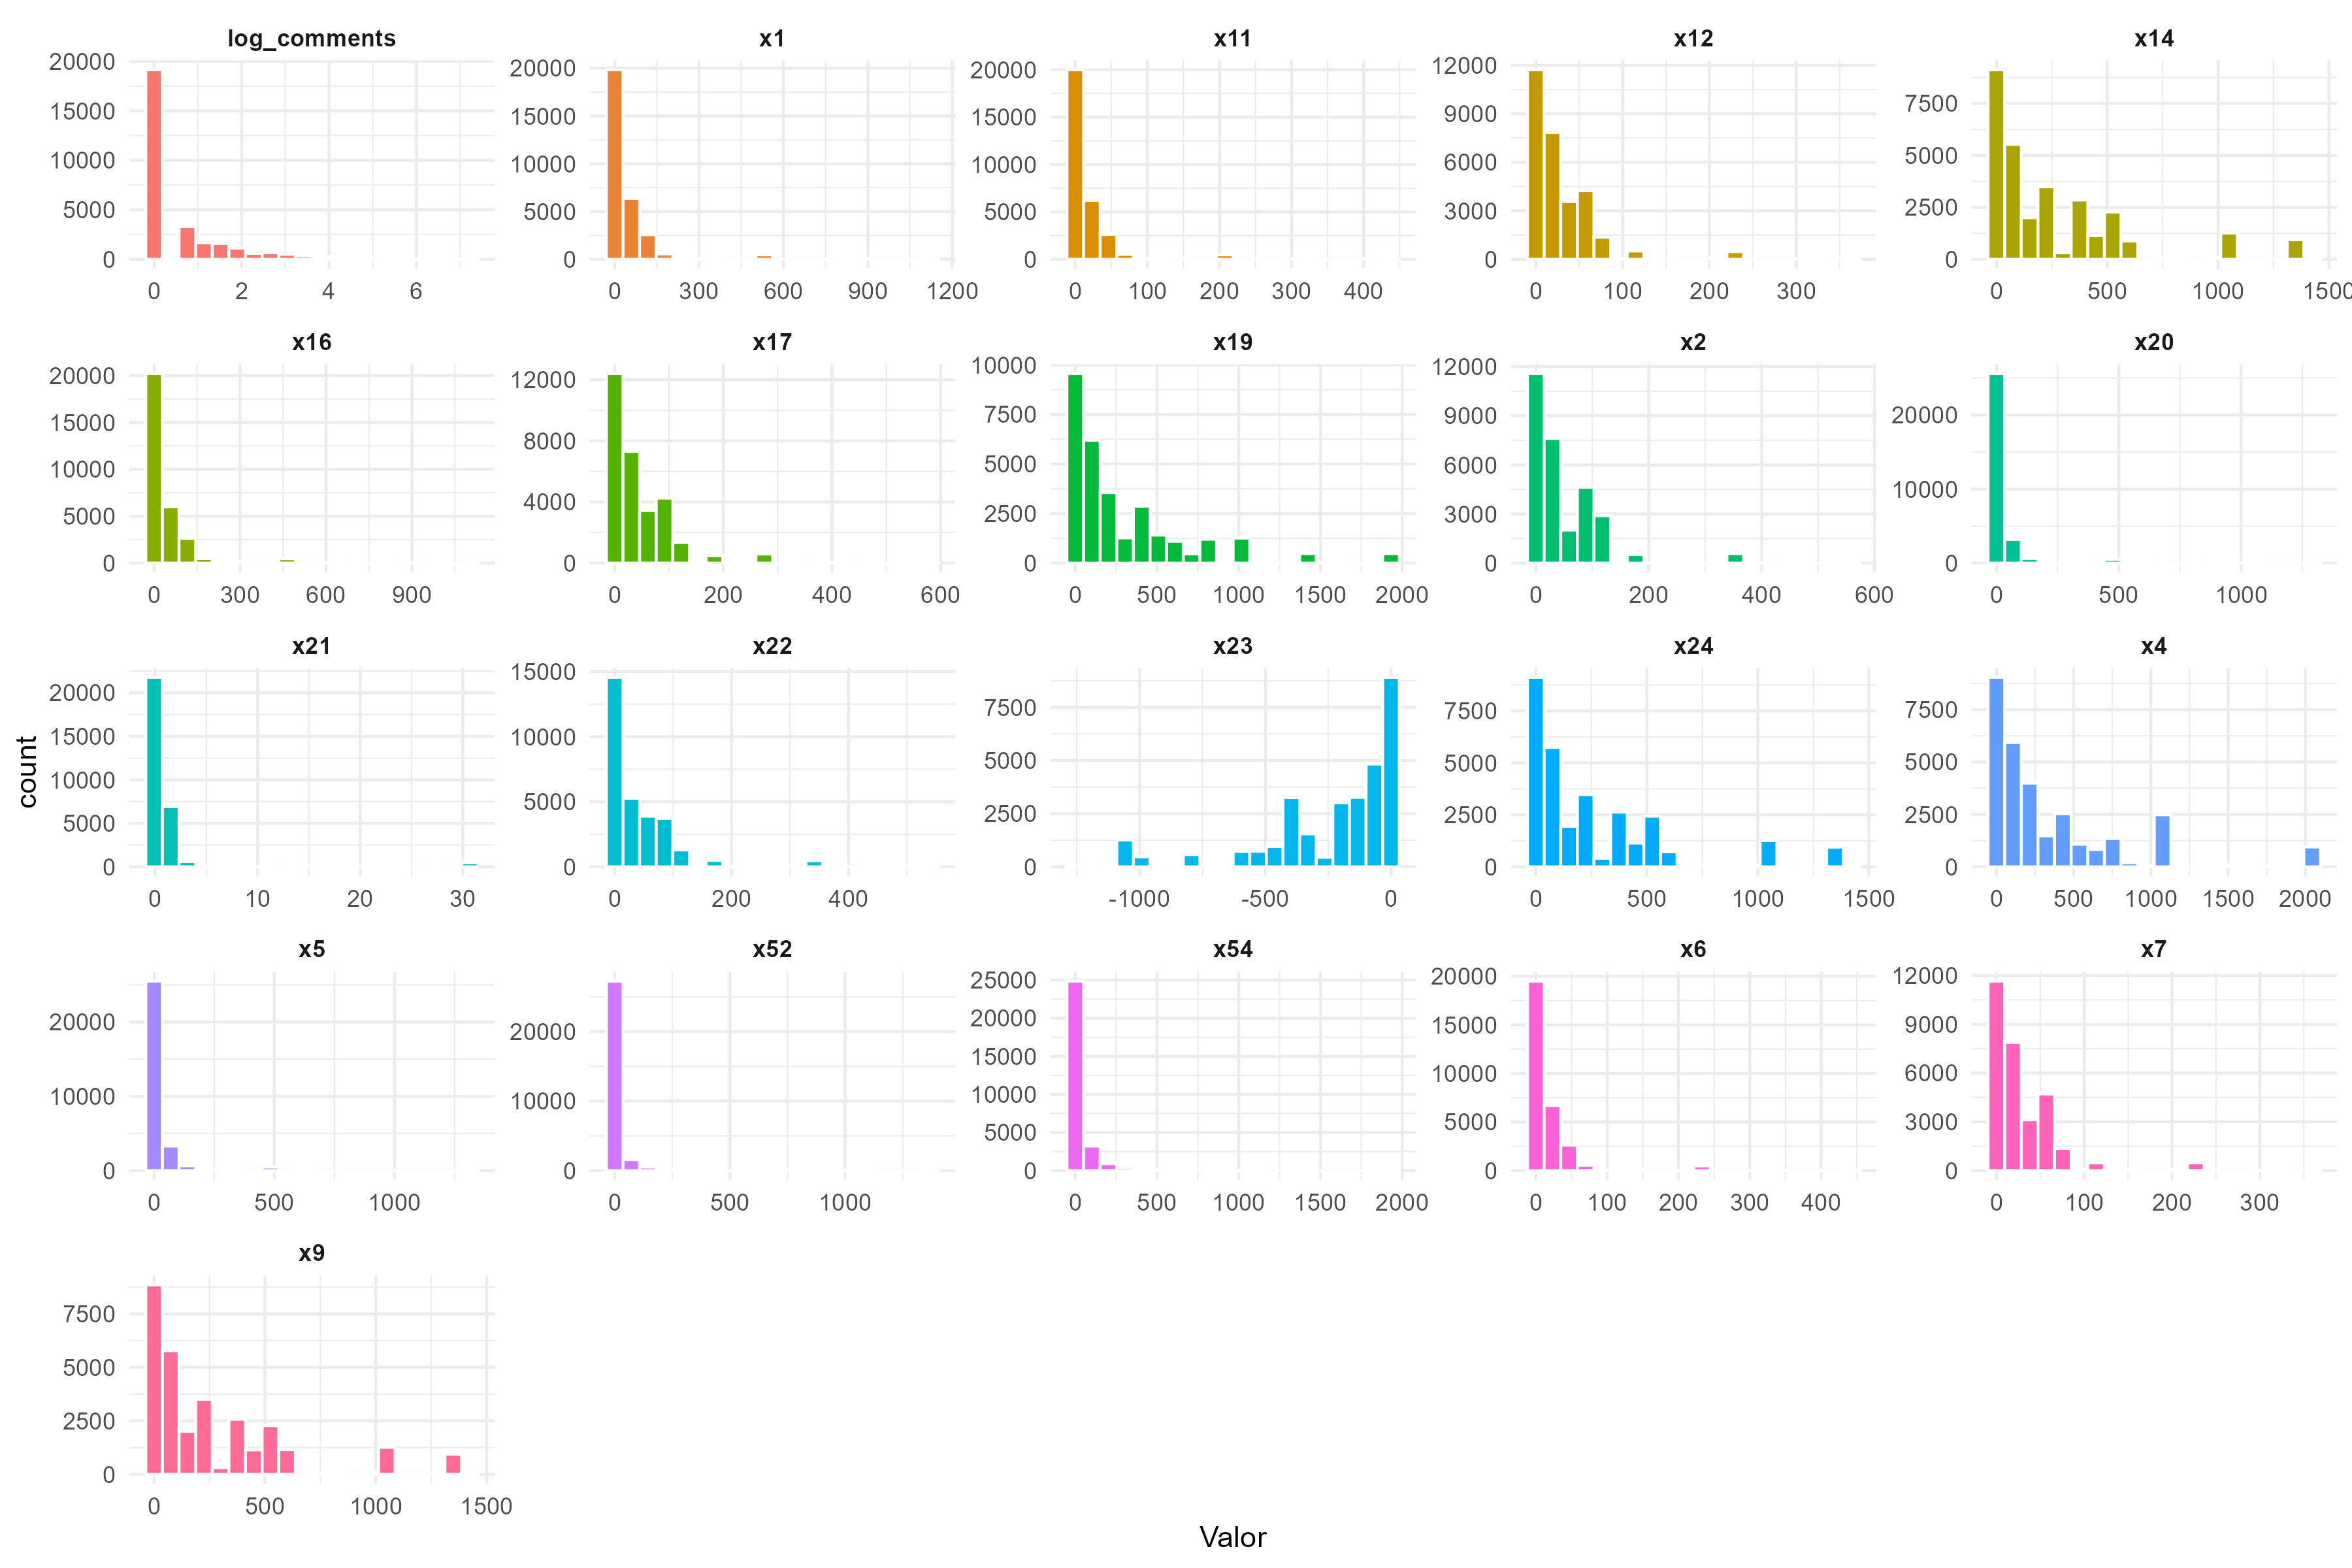
\includegraphics[width=0.95\textwidth]{histogramas_variables.png}
    \caption{Histogramas de las variables seleccionadas.}
    \label{fig:histogramas_variables}
\end{figure}

De los histogramas de la Figura \ref{fig:histogramas_variables}, se observa que las variables presentan distribuciones similares, con grandes colas hacia la derecha, al igual que la variable respuesta, lo que sugiere que los datos están sesgados positivamente, a excepción de la variable x23, que presenta una cola hacia la izquierda, explicando un sesgo negativo.

\newpage

\section{Análisis de Componentes Principales (PCA)}

Aplicamos PCA sobre las variables predictoras estandarizadas con el fin de reducir la dimensionalidad del conjunto de datos y visualizar la relación entre las variables. En la Figura \ref{fig:scree_plot} se muestra el Scree Plot, que representa la varianza explicada por cada componente principal en función del número de componentes.

\begin{figure}[H]
    \centering
    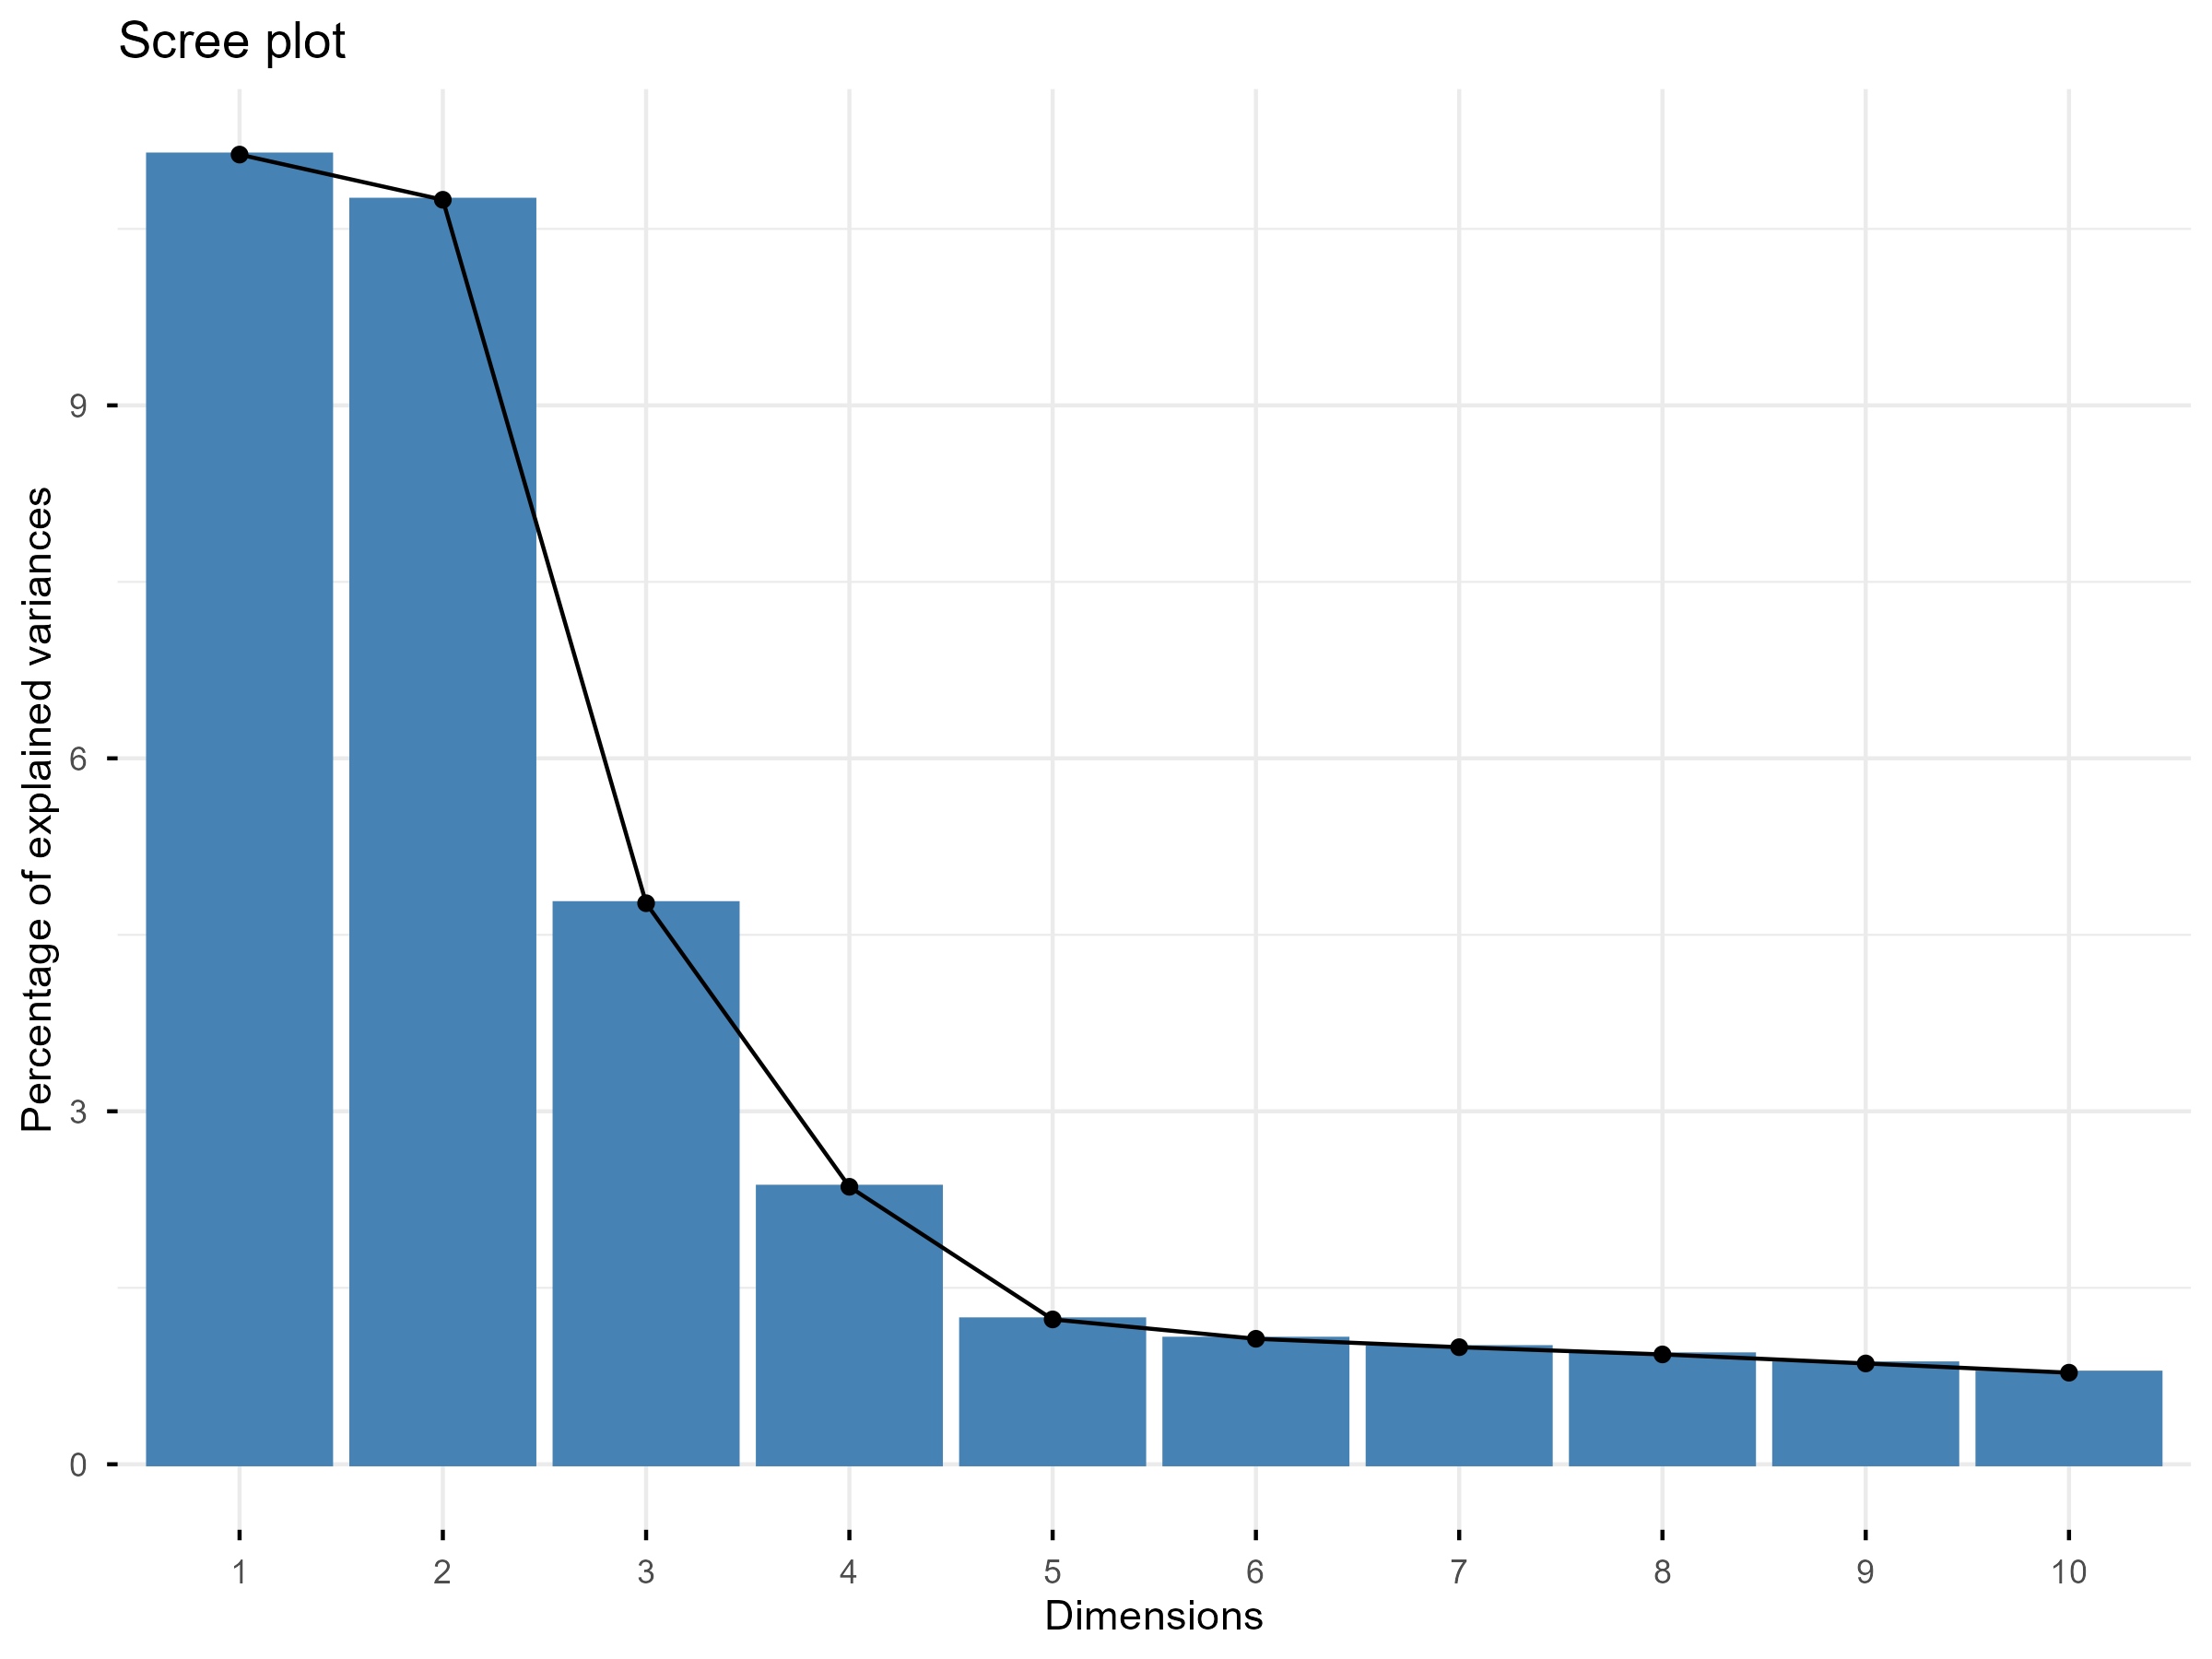
\includegraphics[width=0.8\textwidth]{screeplot_pca.png}
    \caption{Scree Plot de los componentes principales.}
    \label{fig:scree_plot}
\end{figure}

Notamos que los dos primeros componentes principales explican aproximadamente un 10\% de la varianza total, seguidas por una disminución marcada en el tercer y cuarto componente. A partir del quinto componente, la contribución marginal de cada dimensión es relativamente baja.

Como queremos retener los componentes que expliquen al menos el 70\% de la varianza total, necesitaremos 93 componentes principales para alcanzar ese umbral, lo que sugiere que la mayoría de la información se distribuye a lo largo de muchas dimensiones.

Por lo tanto, se puede concluir que no existe redundancia significativa entre bloques de variables, lo que se refleja en la ausencia de un pequeño número de componentes que capture la mayor parte de la varianza, como se demostró anteriormente en el Scree Plot.

La Figura \ref{fig:cargas_pca} muestra las cargas de los dos primeros PCA:

\begin{figure}[H]
    \centering
    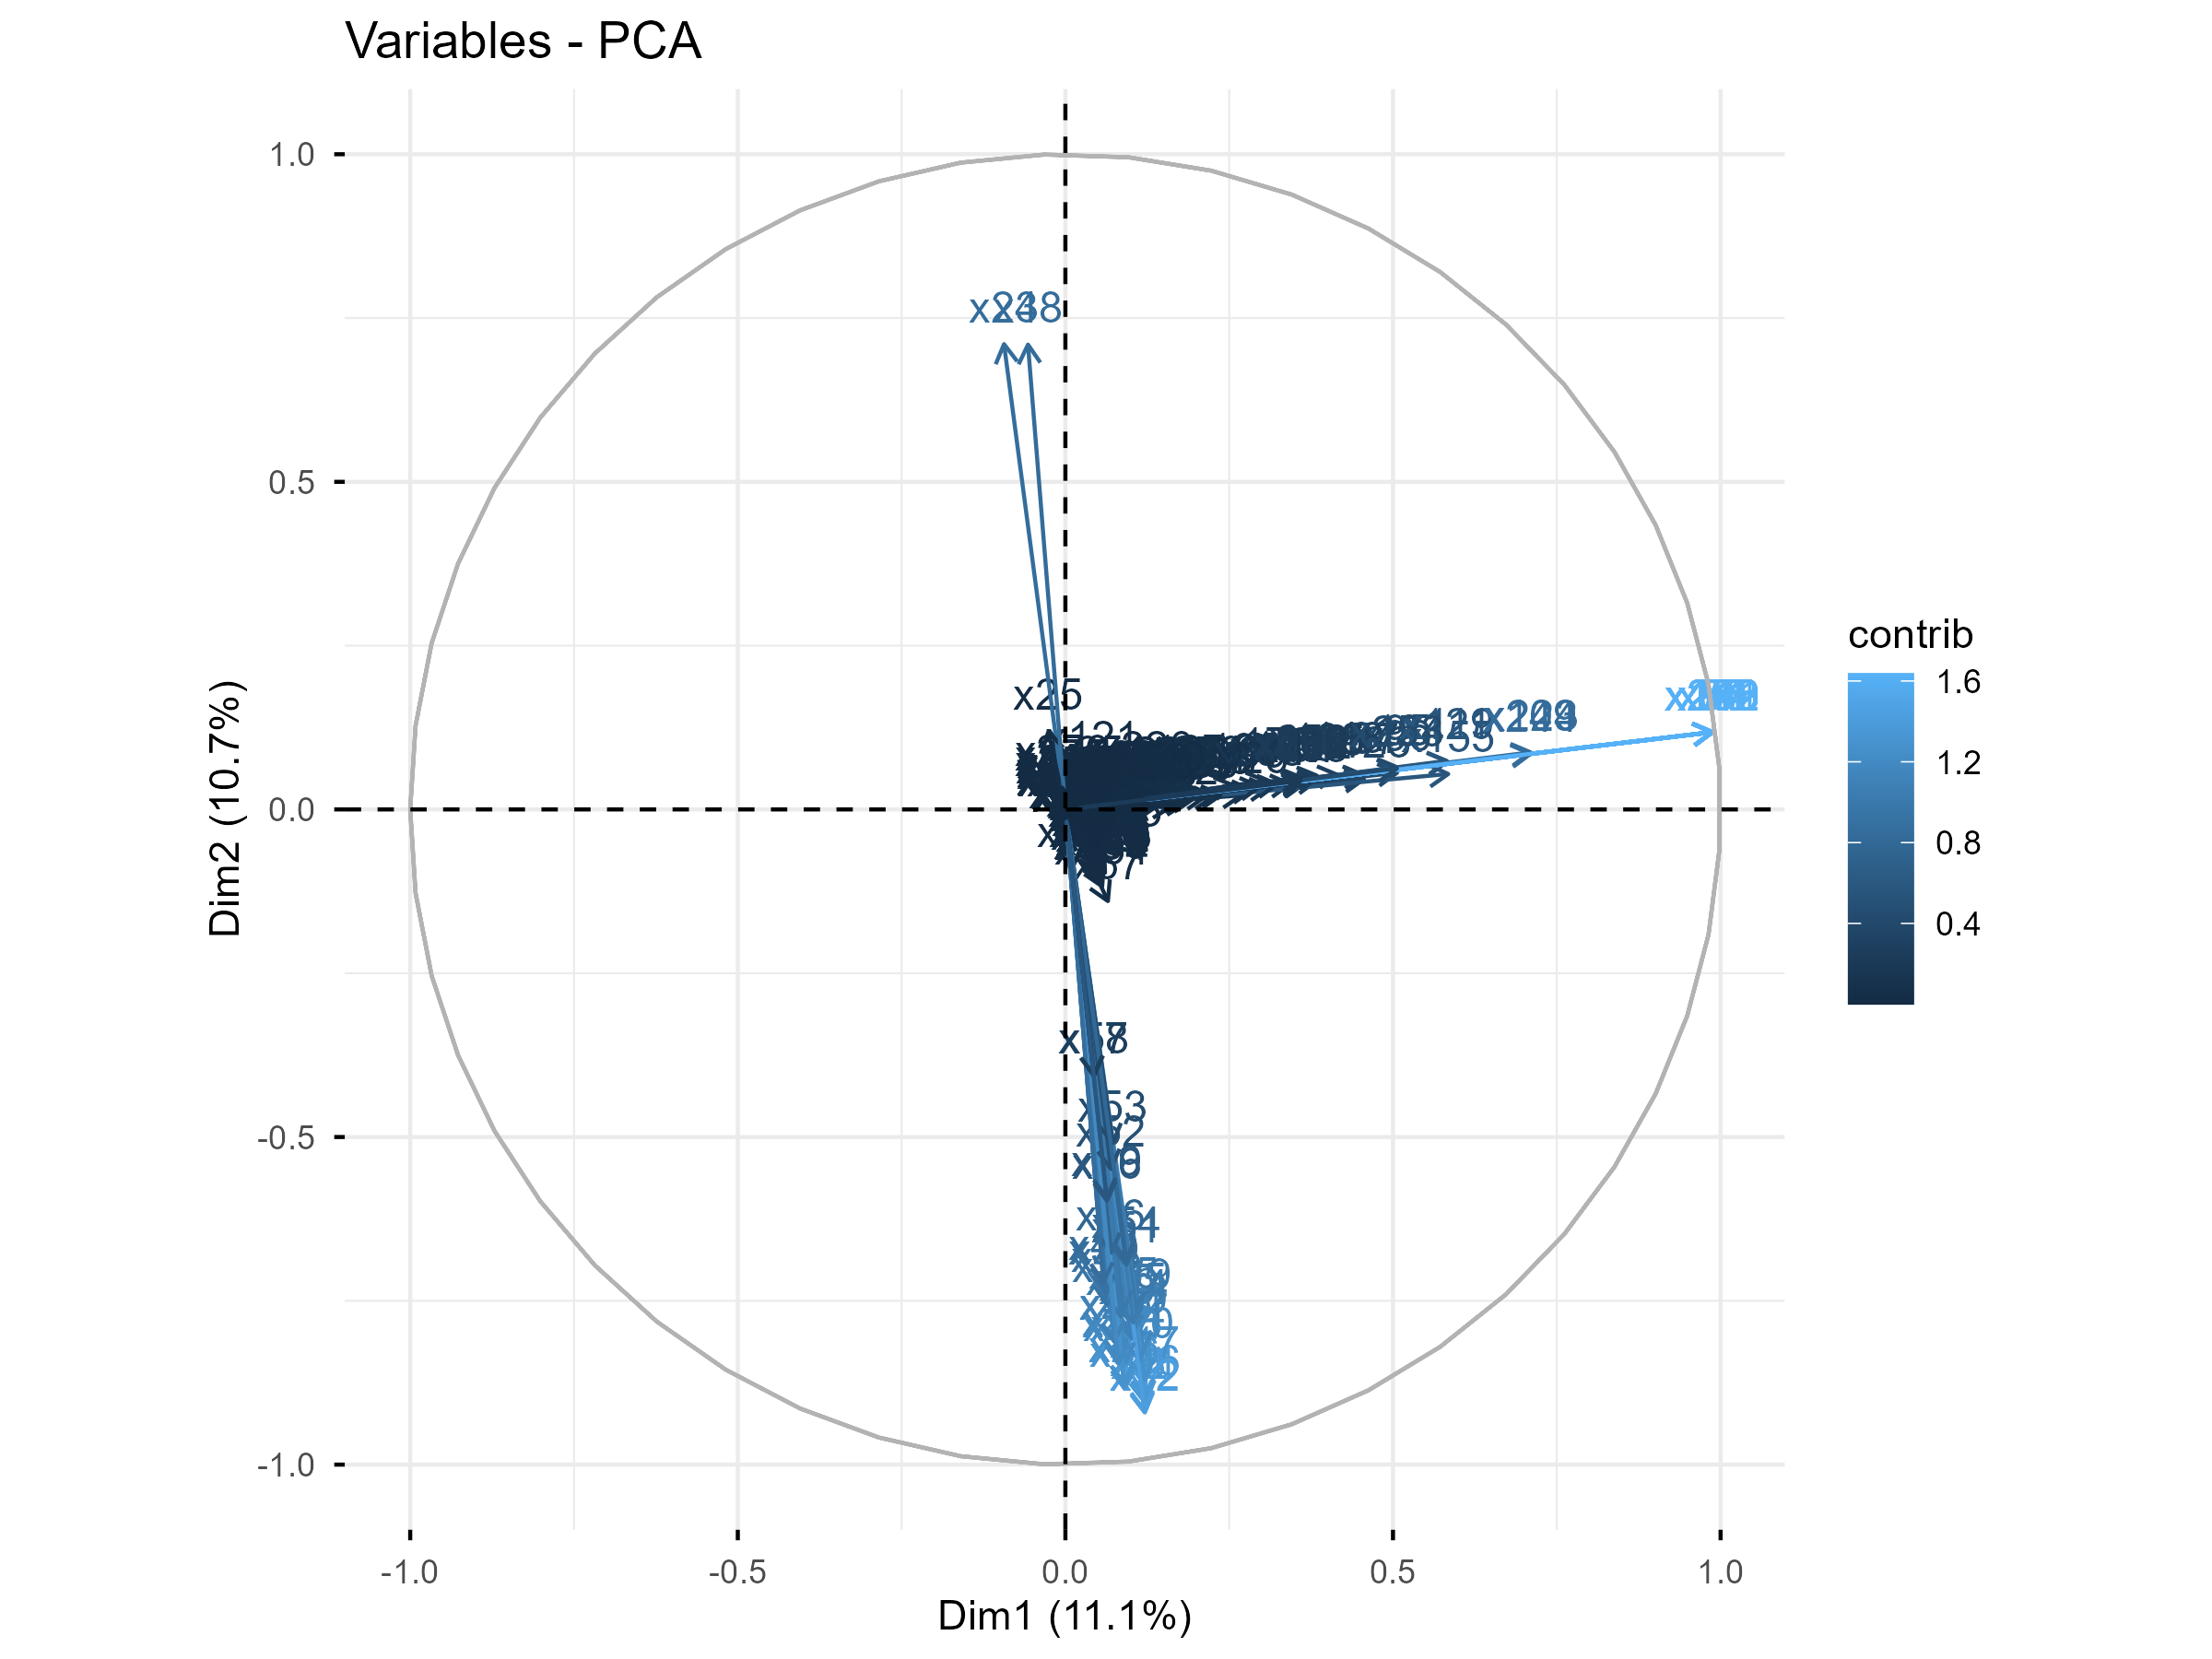
\includegraphics[width=0.65\textwidth]{pca_variables_contrib.png}
    \caption{Cargas de los dos primeros componentes principales.}
    \label{fig:cargas_pca}
\end{figure}

Vemos que el primer componente principal (Dim1) está dominado por un conjunto amplio de variables con cargas positivas, lo que sugiere que captura un nivel general de actividad o intensidad en los datos. Por otro lado, el segundo componente principal (Dim2) está mayoritariamente dominado por un conjunto de variables con carga negativa, pero también presenta un contraste por algunas variables con carga positiva, diferenciando patrones opuestos dentro del conjunto de datos.

En la Figura \ref{fig:varianza_acumulada_pca} se muestra la varianza explicada acumulada por los componentes principales. La linea punteada representa el umbral del 70\% de varianza explicada.

\begin{figure}[H]
    \centering
    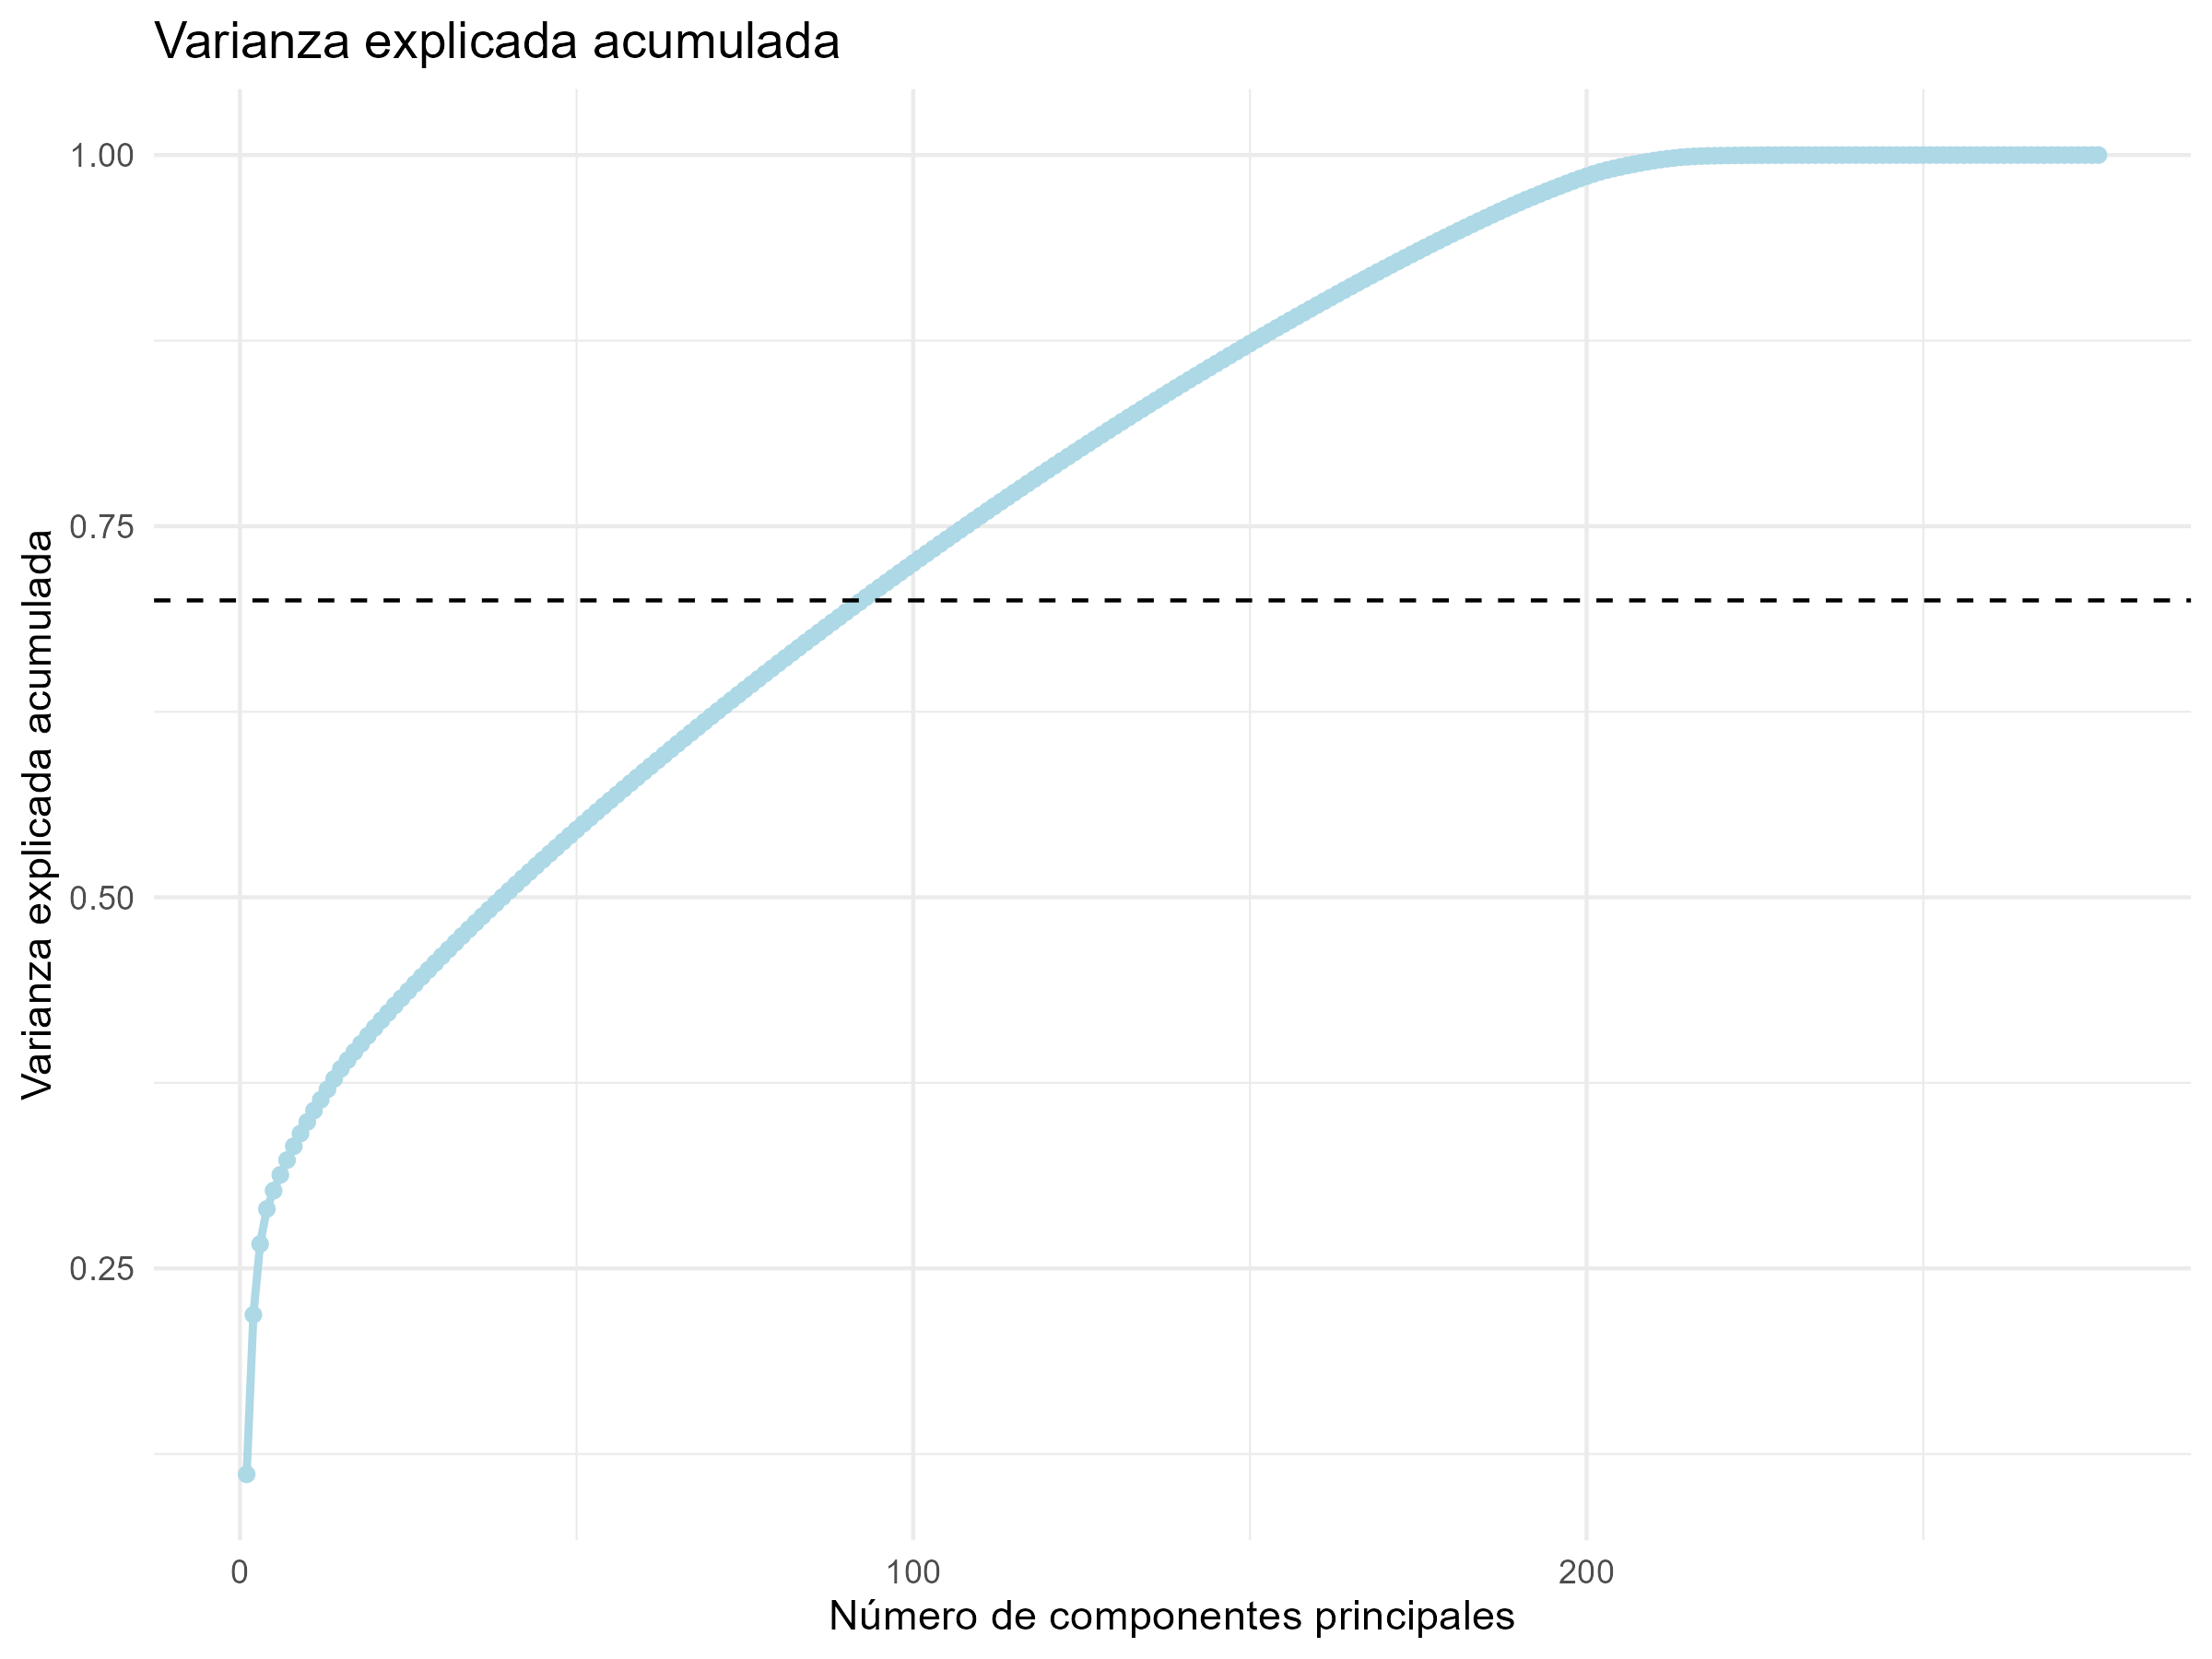
\includegraphics[width=0.65\textwidth]{varianza_acumulada_pca.png}
    \caption{Varianza explicada acumulada por los componentes principales.}
    \label{fig:varianza_acumulada_pca}
\end{figure}

Vemos que la varianza explicada acumulada aumenta lentamente a medida que se añaden más componentes, lo que indica que la información está distribuida a lo largo de muchas dimensiones. Por lo tanto, no hay un pequeño número de componentes que capture la mayor parte de la varianza, como se demostró anteriormente en el Scree Plot.

Realizamos el Biplot de los dos primeros componentes principales junto con las 40 variables que más contribuyen al plano PCA.

\begin{figure}[H]
    \centering
    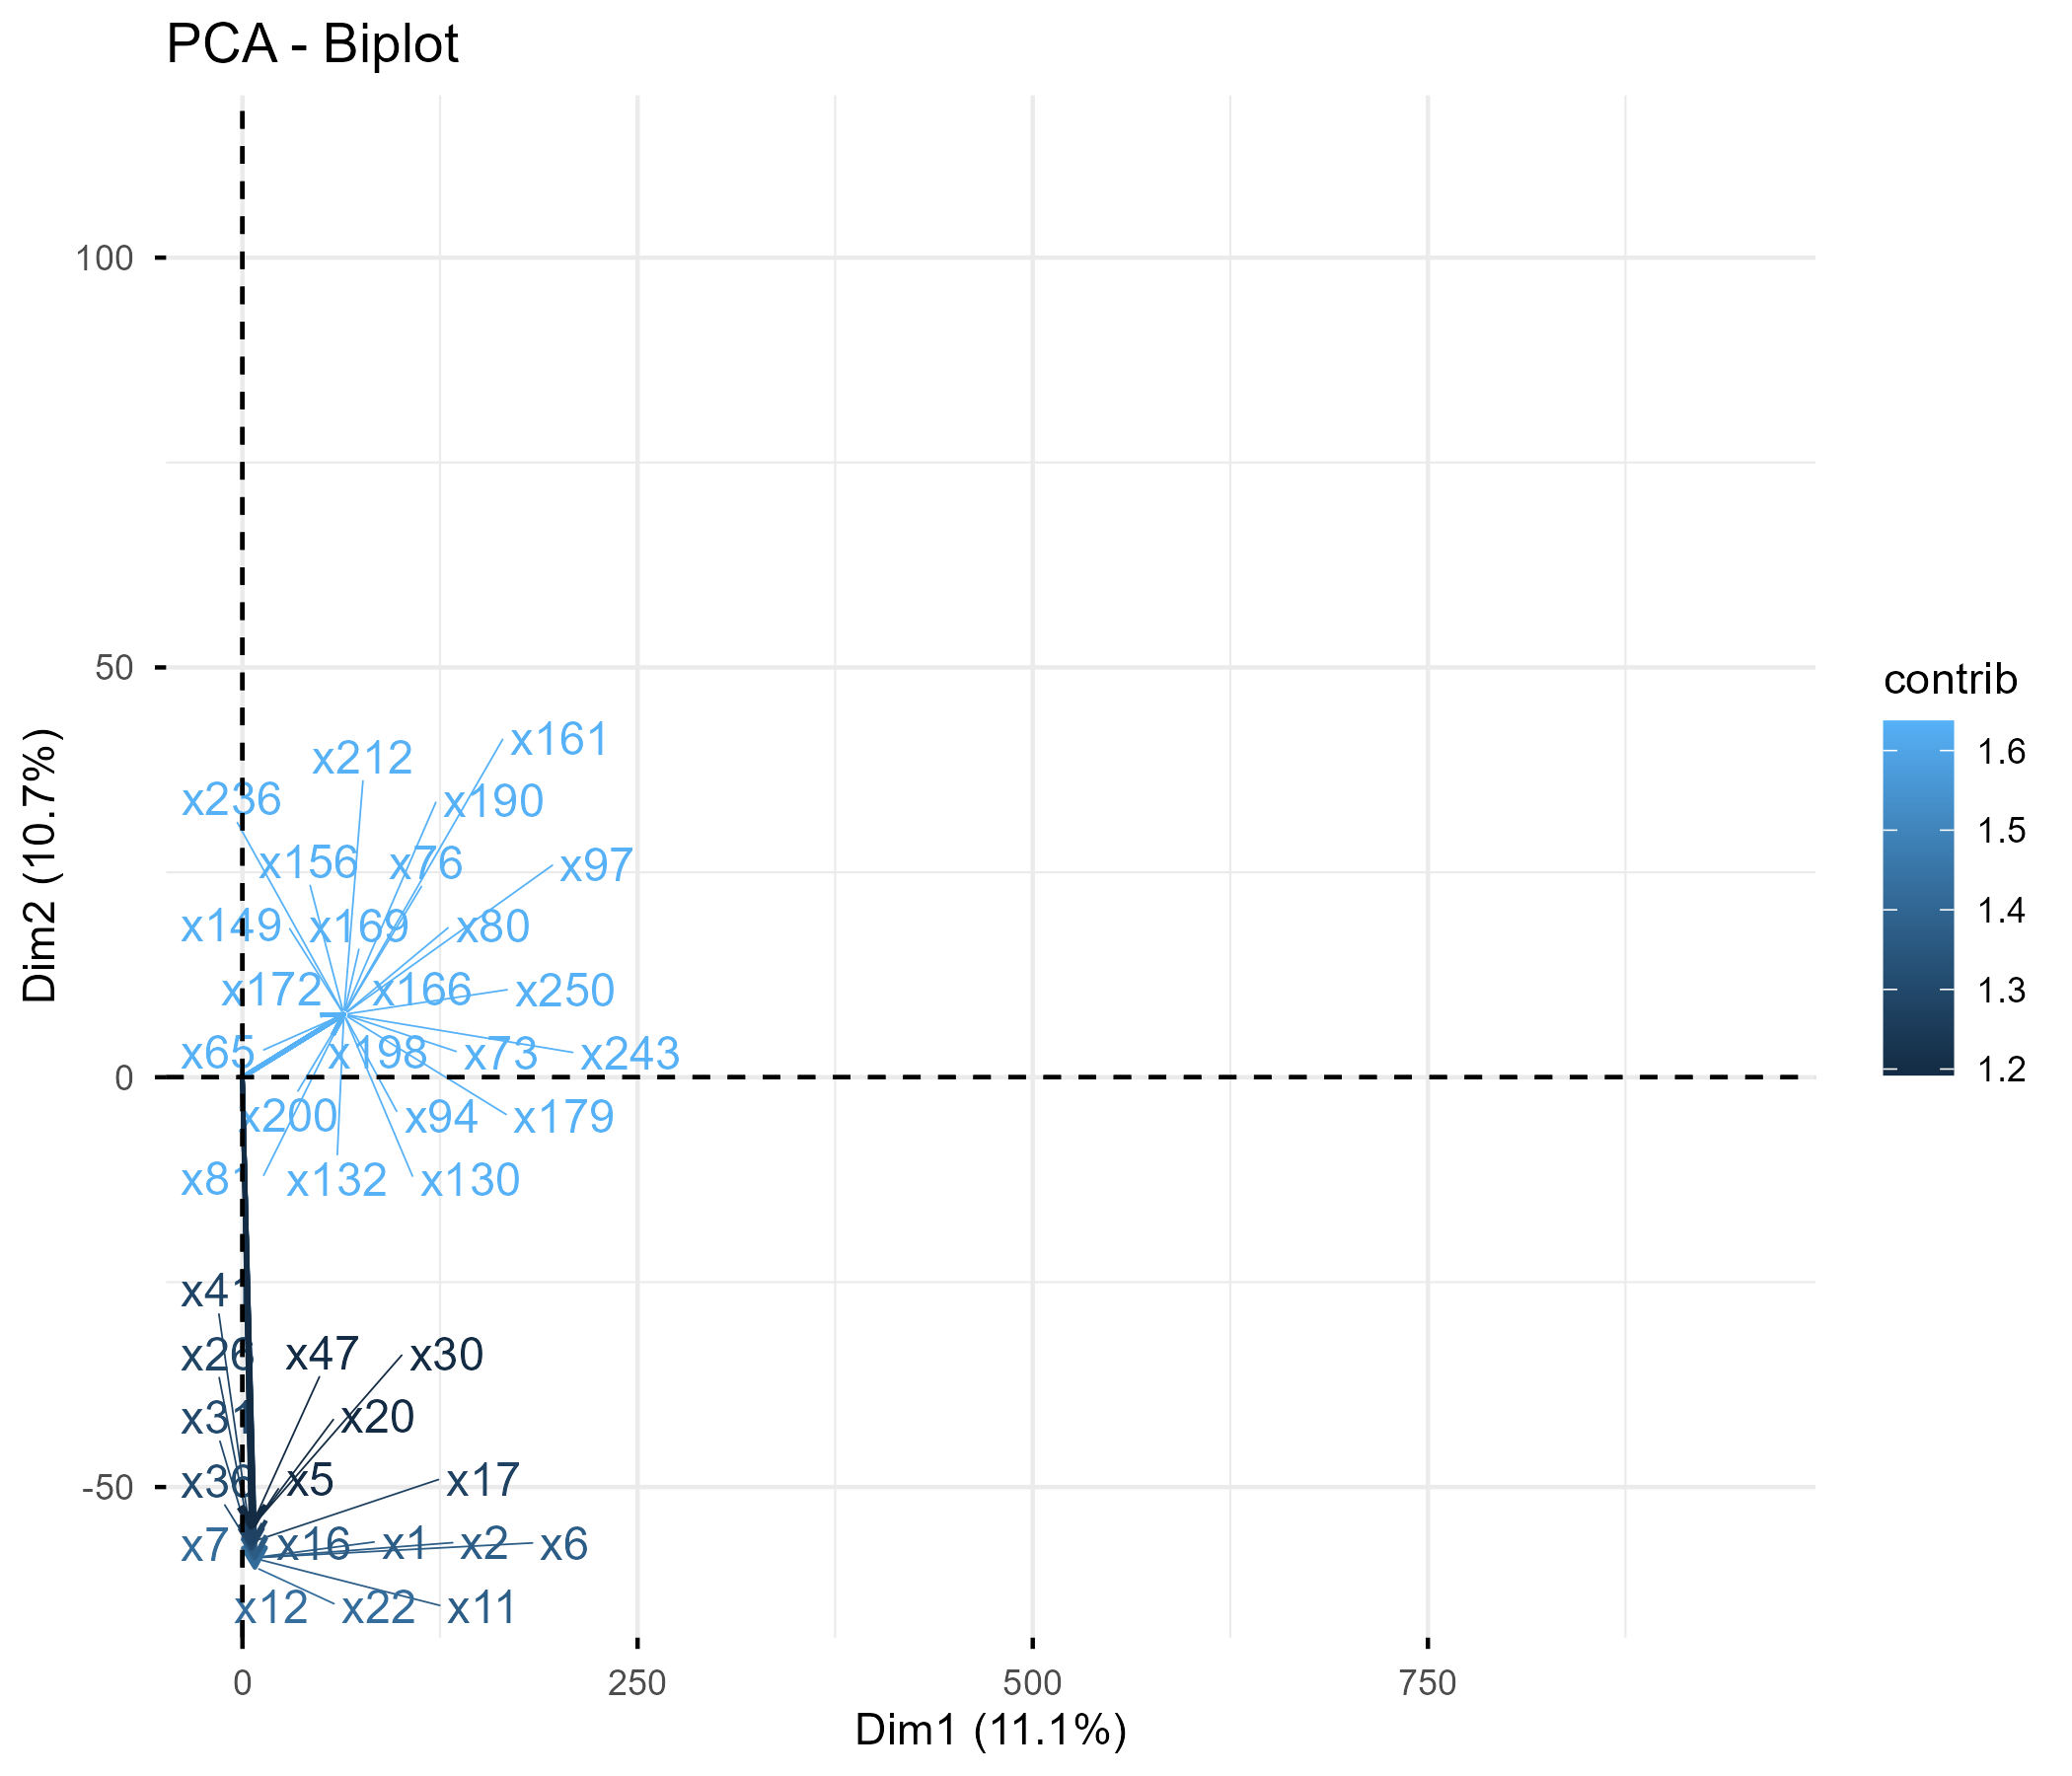
\includegraphics[width=0.75\textwidth]{biplot_pca_contrib40.png}
    \caption{Biplot de los dos primeros componentes principales.}
    \label{fig:biplot_pca}
\end{figure}

El Biplot de la Figura \ref{fig:biplot_pca} muestra que las variables con cargas más altas en el primer componente principal (Dim1) están agrupadas mayoritariamente a valores positivos, mientras que las variables con cargas más altas en el segundo componente principal (Dim2) están agrupadas hacia valores negativos. Se puede concluir que el primer componente captura un patrón general de actividad, mientras que el segundo componente diferencia entre patrones opuestos dentro del conjunto de datos.

\newpage

\section{Modelos de regresión}

Se ajustaron modelos OLS, Lasso y Ridge utilizando las variables predictoras seleccionadas. Además, se estimaron versiones alternativas de estos modelos empleando componentes principales, con el fin de comparar su desempeño predictivo. Para la selección del parámetros de penalización, se utilizó validación cruazada. En la Tabla \ref{fig:modelos} se presentan los resultados de los modelos ajustados, incluyendo el error cuadrático medio (MSE) de validación.

\begin{figure}[H]
    \centering
    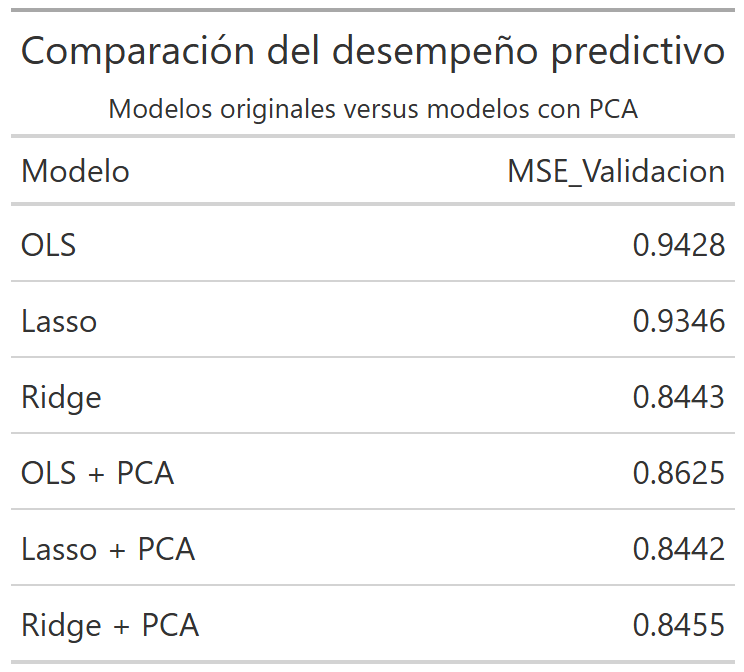
\includegraphics[width=0.5\textwidth]{tabla_mse_modelos.png}
    \caption{Resultados de los modelos de regresión ajustados.}
    \label{fig:modelos}
\end{figure}

Notamos que los modelos de regresión que utilizan componentes principales presentan un desempeño predictivo superior en comparación con los modelos que contienen todas las variables predictoras, por lo tanto la reducción de dimensionalidad a través de PCA ha permitido mejorar la capacidad de generalización de los modelos en general, descartando el modelo Ridge sin PSA, que presenta un desempeño similar al modelo Lasso con PSA y siendo incluso mejor que el modelo Ridge con PSA.

En modelo OLS sin PSA presenta el peor desempeño, lo que sugiere que la inclusión de todas las variables predictoras sin reducción de dimensionalidad puede llevar a un sobreajuste y a una menor capacidad de generalización.

Finalmente, el modelo Lasso con PSA y Ridge con las variables predictoras presentan el mejor desempeño. Esto se explica, ya que el modelo Lasso con PSA se beneficia de la reducción de dimensionalidad, lo que permite una mejor selección de variables y una mayor capacidad de generalización. Por otro lado, el modelo Ridge con las variables predictoras se beneficia por la regularización, lo que permite reducir el sobreajuste y a mejorar la capacidad de generalización.

En la Tabla \ref{fig:coeficientes_lasso} se presentan las primeras 10 variables más relevantes según los coeficientes finales de Lasso con todas las variables predictoras.

\begin{figure}[H]
    \centering
    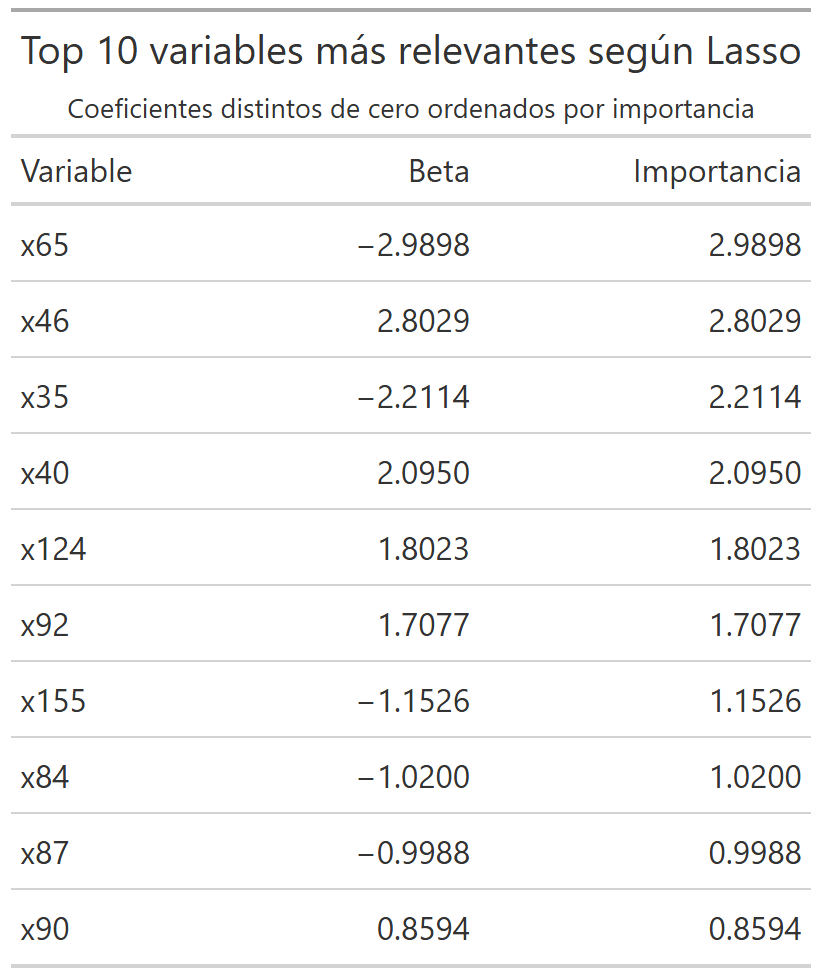
\includegraphics[width=0.5\textwidth]{tabla_top10_lasso.png}
    \caption{Variables más relevantes según los coeficientes finales de Lasso con todas las variables predictoras.}
    \label{fig:coeficientes_lasso}
\end{figure}

Se observa que las variables x65, x46, x35 y x40 son las variables con mayor importancia relativa en el modelo Lasso, demostrando efectos negativos como positivos sobre la variables respuesta \texttt{log\_comments}.

\newpage

\section{Discusión final}

En contextos de alta dimensionalidad, como el presente caso, los modelos de regresión como OLS pueden enfrentar problemas de sobreajuste debido a la gran cantidad de variables predictoras en relación con el número de observaciones. Esto puede llevar a un desempeño predictivo deficiente en la muestra de validación. Por otro lado, los modelos de regresión regularizados como Lasso y Ridge introducen penalizaciones que ayudan a reducir el sobreajuste, ya que limitan la magnitud de los coeficientes, lo que puede mejorar la capacidad de generalización. Además, la aplicación de técnicas de reducción de dimensionalidad como PCA puede ayudar a capturar la información más relevante en un espacio de menor dimensión, lo que también puede mejorar el desempeño predictivo de los modelos.

Es importante respetar la partición temporal de los datos, ya que esto refleja la realidad de la predicción en un contexto temporal, donde se busca predecir eventos futuros basándose en información pasada. Romper esta partición temporal podría llevar a una evaluación optimista del desempeño del modelo, ya que se estaría utilizando información del futuro para predecir el pasado, lo que no es representativo de la situación real. Además, la partición temporal permite evaluar la capacidad del modelo para generalizar a datos no vistos, lo que es fundamental para la utilidad práctica del modelo en escenarios de predicción. \footnote{Para la realización de esta tarea se utilizó inteligencia artificial para mejorar la redacción y claridad de los resultados obtenidos.}

\end{document}
